% =====================================================================
% ELMED219: Kunstig intelligens og beregningsorientert medisin
% Emnebeskrivelse og momentliste - Våren 2026
% =====================================================================
\documentclass[11pt,a4paper]{article}

% =====================================================================
% PAKKER
% =====================================================================
\usepackage[utf8]{inputenc}
\usepackage[T1]{fontenc}
\usepackage[norsk]{babel}
\usepackage{graphicx}
\usepackage{booktabs}
\usepackage{longtable}
\usepackage{tabularx}
\usepackage{array}
\usepackage{multirow}
\usepackage{xcolor}
\usepackage{hyperref}
\usepackage{enumitem}
\usepackage{geometry}
\usepackage{fancyhdr}
\usepackage{titlesec}
\usepackage{tcolorbox}
\usepackage{amsmath}
\usepackage{amssymb}
\usepackage{natbib}
\usepackage{tikz}
\usetikzlibrary{shapes.geometric, arrows, positioning, mindmap}
\usepackage{multicol}

% =====================================================================
% LAYOUT OG FORMATERING
% =====================================================================
\geometry{margin=2.5cm}
\setlength{\parindent}{0pt}
\setlength{\parskip}{0.5em}

% Farger
\definecolor{uibblue}{RGB}{0, 61, 115}
\definecolor{uibred}{RGB}{175, 28, 44}
\definecolor{lightgray}{RGB}{245, 245, 245}
\definecolor{corecolor}{RGB}{0, 100, 0}
\definecolor{recommendedcolor}{RGB}{0, 0, 150}
\definecolor{optionalcolor}{RGB}{100, 100, 100}

% Hyperref
\hypersetup{
    colorlinks=true,
    linkcolor=uibblue,
    citecolor=uibblue,
    urlcolor=uibred
}

% Tittelformatering
\titleformat{\section}{\Large\bfseries\color{uibblue}}{\thesection}{1em}{}
\titleformat{\subsection}{\large\bfseries\color{uibblue!80}}{\thesubsection}{1em}{}
\titleformat{\subsubsection}{\normalsize\bfseries\color{uibblue!60}}{\thesubsubsection}{1em}{}

% Header/Footer
\pagestyle{fancy}
\fancyhf{}
\fancyhead[L]{\small\textcolor{gray}{ELMED219 -- Våren 2026}}
\fancyhead[R]{\small\textcolor{gray}{Emnebeskrivelse og momentliste}}
\fancyfoot[C]{\thepage}
\renewcommand{\headrulewidth}{0.4pt}

% Boksdefinisjoner
\newtcolorbox{infobox}[1][]{
    colback=lightgray,
    colframe=uibblue,
    title=#1,
    fonttitle=\bfseries,
    boxrule=0.5pt
}

\newtcolorbox{warningbox}[1][]{
    colback=uibred!5,
    colframe=uibred,
    title=#1,
    fonttitle=\bfseries,
    boxrule=0.5pt
}

% =====================================================================
% DOKUMENT START
% =====================================================================
\begin{document}

% =====================================================================
% TITTELSIDE
% =====================================================================
\begin{titlepage}
\centering
\vspace*{0.5cm}

{\Huge\bfseries\color{uibblue} ELMED219}\\[0.3cm]
{\Large\bfseries Kunstig intelligens og beregningsorientert medisin}\\[0.6cm]

\rule{\textwidth}{1pt}\\[0.3cm]
{\LARGE Emnebeskrivelse og momentliste}\\[0.2cm]
{\large Våren 2026}\\[0.3cm]
\rule{\textwidth}{1pt}

\vspace{1cm}

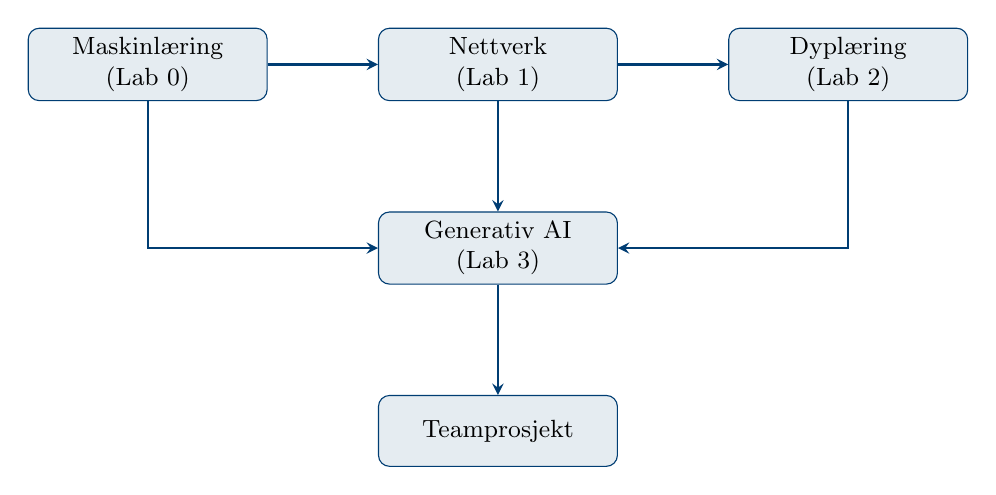
\begin{tikzpicture}[node distance=1.4cm, auto]
    % Styles
    \tikzstyle{block} = [rectangle, draw=uibblue, fill=uibblue!10, 
        text width=2.8cm, text centered, rounded corners, minimum height=0.9cm, font=\small]
    \tikzstyle{arrow} = [thick,->,>=stealth,uibblue]
    
    % Nodes
    \node [block] (ml) {Maskinlæring\\(Lab 0)};
    \node [block, right=of ml] (net) {Nettverk\\(Lab 1)};
    \node [block, right=of net] (dl) {Dyplæring\\(Lab 2)};
    \node [block, below=of net] (genai) {Generativ AI\\(Lab 3)};
    \node [block, below=of genai] (team) {Teamprosjekt};
    
    % Arrows
    \draw [arrow] (ml) -- (net);
    \draw [arrow] (net) -- (dl);
    \draw [arrow] (ml) |- (genai);
    \draw [arrow] (dl) |- (genai);
    \draw [arrow] (net) -- (genai);
    \draw [arrow] (genai) -- (team);
\end{tikzpicture}

\vspace{1cm}

{\large
\textbf{Institutt for biomedisin}\\
Det medisinske fakultet\\
Universitetet i Bergen\\[0.5cm]
I samarbeid med\\
Mohn Medical Imaging and Visualization Center (MMIV)
}

\vspace{0.8cm}

\rule{0.6\textwidth}{0.4pt}

\vspace{0.5cm}

{\normalsize
\textbf{Kursansvarlig:} Arvid Lundervold\\[0.2cm]
\textbf{Kursmateriale:} \url{https://github.com/arvidl/ELMED219-2026}
}

\vfill
{\footnotesize Desember 2025}

\end{titlepage}

% =====================================================================
% INNHOLDSFORTEGNELSE
% =====================================================================
\tableofcontents
\newpage

% =====================================================================
% 1. INNLEDNING OG MOTIVASJON
% =====================================================================
\section{Innledning og motivasjon}

\subsection{Hvorfor AI i medisin?}

Kunstig intelligens (AI) og maskinlæring transformerer i økende grad helsetjenester og biomedisinsk forskning \citep{topol2019high}. Fra bildediagnostikk og prediksjon av sykdomsforløp til klinisk beslutningsstøtte og legemiddelutvikling -- AI-baserte verktøy blir stadig mer relevante for helsepersonell og forskere.

\begin{infobox}[Kursets kjernespørsmål]
\begin{itemize}[nosep]
    \item Hvordan fungerer maskinlæring og dyplæring?
    \item Hvordan kan AI anvendes ansvarlig i medisin?
    \item Hvilke muligheter og begrensninger har dagens AI-teknologi?
    \item Hva betyr \emph{presisjonsmedisin} i praksis?
\end{itemize}
\end{infobox}

\subsection{Emnets plass i utdanningen}

ELMED219 er et valgfritt emne på 5 studiepoeng som tilbys til medisinstudenter og andre med interesse for AI i helsekontekst. Kurset er delt med BMED365 (Computational imaging, modelling and AI in biomedicine), som går over to blokker.

\subsection{Læringsutbytte}

Etter fullført emne skal studenten kunne:

\subsubsection*{Kunnskap}
\begin{itemize}[nosep]
    \item Forklare grunnleggende prinsipper for maskinlæring, dyplæring og generativ AI
    \item Beskrive nettverksanalyse og pasient-likhetsnettverk (PSN)
    \item Gjøre rede for etiske og regulatoriske aspekter ved medisinsk AI
    \item Forstå konsepter som \emph{forklarbar AI} (XAI) og \emph{trustworthy AI}
\end{itemize}

\subsubsection*{Ferdigheter}
\begin{itemize}[nosep]
    \item Anvende Python og Jupyter Notebooks for enkle ML-analyser
    \item Bruke AI-verktøy (ChatGPT, Gemini, Claude) som lærings- og arbeidspartnere
    \item Konstruere og analysere pasient-likhetsnettverk
    \item Skrive en forskningsplan med LaTeX
\end{itemize}

\subsubsection*{Generell kompetanse}
\begin{itemize}[nosep]
    \item Vurdere muligheter og begrensninger ved AI i klinisk praksis
    \item Reflektere over etiske implikasjoner av AI-teknologi
    \item Samarbeide tverrfaglig i prosjektgrupper
    \item Kommunisere faglig om AI-relaterte temaer
\end{itemize}

% =====================================================================
% 2. KURSSTRUKTUR OG INNHOLD
% =====================================================================
\section{Kursstruktur og innhold}

\subsection{Oversikt over aktiviteter}

Kurset er organisert rundt fire laboratorier (Labs), et lynkurs og et teamprosjekt. Tabell~\ref{tab:aktiviteter} gir en oversikt.

\begin{table}[htbp]
\centering
\caption{Oversikt over kursaktiviteter}
\label{tab:aktiviteter}
\begin{tabular}{@{}llp{6cm}c@{}}
\toprule
\textbf{Aktivitet} & \textbf{Tema} & \textbf{Beskrivelse} & \textbf{Timer} \\
\midrule
Lynkurs & AI-assistert Python & Intro til Python og AI-verktøy & 4 \\
Lab 0 & Maskinlæring & ML med scikit-learn og PyCaret & 6 \\
Lab 1 & Nettverksvitenskap & Grafteori og PSN med NetworkX & 6 \\
Lab 2 & Dyplæring & CNN og nevrale nettverk med PyTorch & 8 \\
Lab 3 & Generativ AI \& LLM & Transformers, prompting, etikk & 6 \\
\midrule
Teamprosjekt & Presisjonsmedisin & Forskningsplan for glioblastom & 15 \\
\bottomrule
\end{tabular}
\end{table}

\subsection{Lynkurs: AI-assistert Python-programmering}

Lynkurset er designet for studenter uten tidligere programmeringserfaring. Det gir en praktisk introduksjon til:

\begin{itemize}[nosep]
    \item Google Colab og Jupyter Notebooks
    \item Python-grunnlag: variabler, datatyper, lister, funksjoner
    \item AI som programmeringspartner (Gemini/ChatGPT)
    \item Smakebit fra Lab 0 (klassifisering) og Lab 1 (nettverk)
\end{itemize}

\subsection{Lab 0: Maskinlæring (ML)}

Lab 0 gir en praktisk innføring i maskinlæring med fokus på klassifisering og evaluering.

\begin{table}[htbp]
\centering
\caption{Notebooks i Lab 0}
\label{tab:lab0}
\begin{tabular}{@{}clp{7cm}@{}}
\toprule
\textbf{Nr} & \textbf{Notebook} & \textbf{Innhold} \\
\midrule
01 & Enkle eksempler & Features, labels, trening, testing, decision trees \\
02 & Binær klassifikasjon & Confusion matrix, ROC, precision, recall, F1-score \\
03 & PyCaret hurtigguide & AutoML for rask prototyping \\
\bottomrule
\end{tabular}
\end{table}

\textbf{Læringsmål:}
\begin{itemize}[nosep]
    \item Skille mellom supervised og unsupervised læring
    \item Bruke train/test split og kryssvalidering
    \item Tolke evalueringsmetrikker (accuracy, precision, recall, AUC)
    \item Forstå TRIPOD-retningslinjer for medisinsk ML
\end{itemize}

\subsection{Lab 1: Nettverksvitenskap og PSN}

Lab 1 introduserer grafteori og konseptet \emph{pasient-likhetsnettverk} (PSN) -- en tilnærming for å identifisere pasientsubgrupper basert på likhet.

\begin{table}[htbp]
\centering
\caption{Notebooks i Lab 1}
\label{tab:lab1}
\begin{tabular}{@{}clp{6.5cm}@{}}
\toprule
\textbf{Nr} & \textbf{Notebook} & \textbf{Innhold} \\
\midrule
00 & Introduksjon & Grafteori, nabomatriser, sentralitetsmål \\
01 & NetworkX tutorial & Opprette, manipulere, visualisere grafer \\
02 & PSN med IRIS & Likhetsberegning, community detection \\
03 & PSN med IBS-data & Klinisk anvendelse: hjerne og kognisjon \\
04 & PSN med IQ-data & WAIS-IV og kognitive profiler \\
\bottomrule
\end{tabular}
\end{table}

\textbf{Læringsmål:}
\begin{itemize}[nosep]
    \item Definere graf, node, kant, og forstå nabomatriser
    \item Beregne sentralitetsmål (degree, betweenness, eigenvector)
    \item Konstruere PSN fra kliniske data
    \item Anvende Louvain-algoritmen for community detection
\end{itemize}

\subsection{Lab 2: Dyplæring (DL)}

Lab 2 utforsker dyplæring med fokus på nevrale nettverk, CNN og medisinsk bildeanalyse.

\begin{table}[htbp]
\centering
\caption{Notebooks i Lab 2 (prioritert)}
\label{tab:lab2}
\begin{tabular}{@{}cclp{5.5cm}@{}}
\toprule
\textbf{Del} & \textbf{Pri} & \textbf{Notebook} & \textbf{Innhold} \\
\midrule
A & 1 & CNN-intro & Konseptuell intro til CNN \\
A & 1 & MNIST-MLP & Din første DL-modell \\
A & 1 & MNIST-CNN & CNN på håndskrevne sifre \\
\midrule
B & 1 & NN-intro & Biologiske vs. kunstige nevroner \\
B & 1 & Læring i NN & Backpropagation, gradient descent \\
B & 1 & Hjertesykdom & Klassifisering fra tabelldata \\
B & 1 & EKG-arytmi & CNN på EKG-signaler \\
\midrule
C & 2 & CNN-arkitektur & Miljøoppsett og arkitektur \\
C & 2 & CNN-trening & Trening og lagring av modell \\
C & 2 & CNN-testing & Evaluering og Grad-CAM (XAI) \\
\midrule
D & 2 & MR-demens & MRI-bildeanalyse for demens \\
\bottomrule
\end{tabular}
\end{table}

\textbf{Prioritetsnivåer:} 1 = kjerne, 2 = anbefalt, 3 = valgfri, 4 = avansert

\textbf{Læringsmål:}
\begin{itemize}[nosep]
    \item Forklare oppbygningen av et nevralt nettverk
    \item Forstå backpropagation og gradient descent
    \item Bygge og trene CNN med PyTorch
    \item Bruke Grad-CAM for å tolke modellbeslutninger
\end{itemize}

\subsection{Lab 3: Generativ AI og Store Språkmodeller}

Lab 3 dekker generativ AI og store språkmodeller (LLM) med fokus på medisinsk anvendelse, etikk og forklarbarhet.

\begin{table}[htbp]
\centering
\caption{Notebooks i Lab 3}
\label{tab:lab3}
\begin{tabular}{@{}ccp{6cm}c@{}}
\toprule
\textbf{Nr} & \textbf{Prioritet} & \textbf{Tema} & \textbf{Tid} \\
\midrule
01 & \textcolor{corecolor}{Kjerne} & Introduksjon til generativ AI & 45 min \\
02 & \textcolor{corecolor}{Kjerne} & Transformer-arkitekturen & 60 min \\
03 & \textcolor{corecolor}{Kjerne} & LLM grunnleggende (tokens, temp.) & 45 min \\
04 & \textcolor{corecolor}{Kjerne} & Prompt engineering & 90 min \\
\midrule
05 & \textcolor{recommendedcolor}{Viktig} & Forklarbar AI (XAI) & 60 min \\
06 & \textcolor{recommendedcolor}{Viktig} & AI-etikk i medisin & 60 min \\
\midrule
07 & \textcolor{optionalcolor}{Valgfri} & Trustworthy AI & 60 min \\
08 & \textcolor{optionalcolor}{Valgfri} & Nevrosymbolsk AI + Agentisk AI & 90 min \\
09 & \textcolor{optionalcolor}{Valgfri} & ChatGPT/Claude API & 60 min \\
\bottomrule
\end{tabular}
\end{table}

\textbf{NB:} Notebook 08 (Nevrosymbolsk AI) inneholder en omfattende \textbf{case study om hjernesvulster (gliom)} som demonstrerer:
\begin{itemize}[nosep]
    \item Nevrosymbolsk klassifikasjon basert på WHO 2021 CNS-klassifikasjon
    \item Integrasjon av MRI-analyse (nevral) med kunnskapsgrafer (symbolsk)
    \item Agentisk AI som orkestrerer klinisk arbeidsflyt
\end{itemize}

\textbf{Læringsmål:}
\begin{itemize}[nosep]
    \item Forklare self-attention og transformer-arkitekturen
    \item Anvende prompt engineering-teknikker (zero-shot, few-shot, CoT)
    \item Vurdere XAI-metoder som SHAP og LIME
    \item Diskutere AI-etikk, bias, og EU AI Act
    \item Forstå nevrosymbolsk integrasjon av nevrale og symbolske metoder
    \item Beskrive agentisk AI og dens rolle i klinisk beslutningsstøtte
\end{itemize}

\subsection{Teamprosjekt: Presisjonsmedisin ved glioblastom}

Teamprosjektet er en sentral del av kurset der studenter i tverrfaglige grupper utarbeider en forskningsplan (søknadsskisse) for et tenkt prosjekt om AI og avbildning ved hjernesvulst.

\begin{warningbox}[Viktig om teamprosjektet]
Oppgaven går ut på å \textbf{skrive en forskningsplan} -- ikke å faktisk gjennomføre prosjektet med koding eller dataanalyse.
\end{warningbox}

\textbf{Fokusområder:}
\begin{enumerate}[nosep]
    \item Bildeteknologier og modaliteter (MRI, PET)
    \item Bildeavledede biomarkører for glioblastom
    \item Maskinlæringsteknikker (segmentering, klassifisering)
    \item Datahåndteringsplan og etiske betraktninger
\end{enumerate}

\begin{infobox}[Relevant bakgrunn: Gliom-casestudien]
Notebook 08 i Lab 3 inneholder en omfattende nevrosymbolsk AI-casestudie for gliomklassifikasjon basert på WHO 2021 CNS-klassifikasjon. Denne demonstrerer:
\begin{itemize}[nosep]
    \item Integrasjon av MRI-segmentering (BraTS) med molekylære markører (IDH, MGMT, 1p/19q)
    \item Kunnskapsgrafer for behandlingsanbefalinger
    \item Agentisk AI for orkestrering av klinisk arbeidsflyt
\end{itemize}
Studenter kan bruke denne som inspirasjon for teamprosjektet.
\end{infobox}

\textbf{Rapportstruktur:}
\begin{itemize}[nosep]
    \item Forskningsplan: 3--5 sider (bakgrunn, mål, metoder, evaluering)
    \item Datahåndteringsplan og etikk: 1.5--2.5 sider
    \item Skrives på engelsk (felles med BMED365)
    \item LaTeX-mal tilgjengelig på Overleaf
\end{itemize}

% =====================================================================
% 3. DETALJERT MOMENTLISTE
% =====================================================================
\section{Detaljert momentliste}

Denne seksjonen gir en utfyllende momentliste organisert etter tema. Momentene er merket med prioritet: \textbf{K} = kjerne (obligatorisk), \textbf{V} = viktig (anbefalt), \textbf{U} = utdypende (valgfritt).

\subsection{Maskinlæring -- grunnleggende konsepter}

\begin{longtable}{@{}clp{9cm}@{}}
\toprule
\textbf{Pri} & \textbf{Nr} & \textbf{Moment} \\
\midrule
\endfirsthead
\multicolumn{3}{c}{\textit{Fortsettelse fra forrige side}} \\
\toprule
\textbf{Pri} & \textbf{Nr} & \textbf{Moment} \\
\midrule
\endhead
\midrule
\multicolumn{3}{r}{\textit{Fortsetter på neste side}} \\
\endfoot
\bottomrule
\endlastfoot
K & M01 & Definere \emph{maskinlæring} og skille fra tradisjonell programmering \\
K & M02 & Forklare forskjellen mellom \emph{supervised} og \emph{unsupervised} læring \\
K & M03 & Beskrive konseptene \emph{features} (input) og \emph{labels} (output) \\
K & M04 & Forklare hvorfor vi deler data i \emph{trenings-} og \emph{testsett} \\
K & M05 & Definere \emph{overfitting} og \emph{underfitting} \\
K & M06 & Forstå \emph{bias-variance trade-off} \\
V & M07 & Beskrive k-fold \emph{kryssvalidering} og dens fordeler \\
V & M08 & Forklare hva en \emph{baseline-modell} er og hvorfor den er viktig \\
K & M09 & Skille mellom \emph{klassifisering} og \emph{regresjon} \\
V & M10 & Kjenne til enkle modeller: beslutningstre, k-NN, logistisk regresjon \\
\end{longtable}

\subsection{Evaluering av ML-modeller}

\begin{longtable}{@{}clp{9cm}@{}}
\toprule
\textbf{Pri} & \textbf{Nr} & \textbf{Moment} \\
\midrule
\endfirsthead
\midrule
\endhead
\midrule
\endfoot
\bottomrule
\endlastfoot
K & E01 & Tolke en \emph{confusion matrix} (forvirringsmatrise) \\
K & E02 & Definere TP, TN, FP, FN i medisinsk kontekst \\
K & E03 & Beregne og tolke \emph{accuracy} (nøyaktighet) \\
K & E04 & Beregne og tolke \emph{precision} (presisjon, PPV) \\
K & E05 & Beregne og tolke \emph{recall/sensitivity} (sensitivitet) \\
K & E06 & Beregne og tolke \emph{specificity} (spesifisitet) \\
V & E07 & Beregne og tolke \emph{F1-score} \\
K & E08 & Forstå ROC-kurven og AUC som mål på modellkvalitet \\
V & E09 & Forklare når accuracy er utilstrekkelig (ubalanserte datasett) \\
V & E10 & Kjenne til TRIPOD-retningslinjer for rapportering \\
\end{longtable}

\subsection{Grafteori og nettverksvitenskap}

\begin{longtable}{@{}clp{9cm}@{}}
\toprule
\textbf{Pri} & \textbf{Nr} & \textbf{Moment} \\
\midrule
\endfirsthead
\midrule
\endhead
\midrule
\endfoot
\bottomrule
\endlastfoot
K & N01 & Definere hva en \emph{graf} er (noder og kanter) \\
K & N02 & Skille mellom \emph{rettet} og \emph{urettet} graf \\
K & N03 & Skille mellom \emph{vektet} og \emph{uvektet} graf \\
K & N04 & Representere en graf som \emph{nabomatrise} (adjacency matrix) \\
K & N05 & Beregne \emph{degree centrality} og tolke resultatet \\
V & N06 & Beregne \emph{betweenness centrality} og tolke resultatet \\
V & N07 & Beregne \emph{eigenvector centrality} og tolke resultatet \\
V & N08 & Forklare \emph{clustering coefficient} \\
V & N09 & Beskrive \emph{community detection} og Louvain-algoritmen \\
K & N10 & Kjenne til NetworkX-biblioteket for Python \\
\end{longtable}

\subsection{Pasient-likhetsnettverk (PSN)}

\begin{longtable}{@{}clp{9cm}@{}}
\toprule
\textbf{Pri} & \textbf{Nr} & \textbf{Moment} \\
\midrule
\endfirsthead
\midrule
\endhead
\midrule
\endfoot
\bottomrule
\endlastfoot
K & P01 & Forklare konseptet \emph{pasient-likhetsnettverk} (PSN) \\
K & P02 & Beskrive hvordan PSN kan støtte \emph{presisjonsmedisin} \\
K & P03 & Beregne likhet mellom pasienter (Euklidsk, Manhattan, Gower) \\
V & P04 & Konstruere et PSN fra en pasient-feature-matrise \\
V & P05 & Velge terskelverdi for kantoppretting i PSN \\
V & P06 & Identifisere pasientsubgrupper via community detection \\
U & P07 & Diskutere fordeler og begrensninger ved PSN-tilnærmingen \\
U & P08 & Kjenne til multimodal PSN (integrering av ulike datatyper) \\
\end{longtable}

\subsection{Nevrale nettverk og dyplæring}

\begin{longtable}{@{}clp{9cm}@{}}
\toprule
\textbf{Pri} & \textbf{Nr} & \textbf{Moment} \\
\midrule
\endfirsthead
\midrule
\endhead
\midrule
\endfoot
\bottomrule
\endlastfoot
K & D01 & Sammenligne biologiske og kunstige nevroner \\
K & D02 & Beskrive oppbygningen av et \emph{multilags perseptron} (MLP) \\
K & D03 & Forklare hva en \emph{aktiveringsfunksjon} er (ReLU, sigmoid) \\
K & D04 & Forstå konseptet \emph{forward propagation} \\
K & D05 & Forklare \emph{backpropagation} på et konseptuelt nivå \\
K & D06 & Forstå \emph{gradient descent} og læringsrate \\
V & D07 & Kjenne til \emph{loss functions} (cross-entropy, MSE) \\
K & D08 & Beskrive et \emph{konvolusjonelt nevralt nettverk} (CNN) \\
K & D09 & Forklare hva et \emph{konvolusjonsfilter} gjør \\
K & D10 & Beskrive \emph{pooling-lag} og deres funksjon \\
V & D11 & Kjenne til \emph{batch normalization} og \emph{dropout} \\
V & D12 & Forstå konseptet \emph{transfer learning} \\
U & D13 & Kjenne til avanserte arkitekturer (ResNet, ViT) \\
\end{longtable}

\subsection{Generativ AI og store språkmodeller}

\begin{longtable}{@{}clp{9cm}@{}}
\toprule
\textbf{Pri} & \textbf{Nr} & \textbf{Moment} \\
\midrule
\endfirsthead
\midrule
\endhead
\midrule
\endfoot
\bottomrule
\endlastfoot
K & G01 & Definere \emph{generativ AI} og skille fra diskriminativ AI \\
K & G02 & Forklare \emph{self-attention}-mekanismen på et konseptuelt nivå \\
K & G03 & Beskrive transformer-arkitekturen (encoder-decoder) \\
K & G04 & Forklare hva \emph{tokens} er og hvordan tokenisering fungerer \\
K & G05 & Forstå konseptet \emph{kontekstvindu} (context window) \\
K & G06 & Forklare hva \emph{temperature} betyr i tekstgenerering \\
K & G07 & Anvende \emph{zero-shot} prompting \\
K & G08 & Anvende \emph{few-shot} prompting \\
V & G09 & Anvende \emph{Chain-of-Thought} (CoT) prompting \\
V & G10 & Beskrive god praksis for \emph{systemprompts} \\
K & G11 & Definere \emph{hallusinering} og dens implikasjoner \\
V & G12 & Kjenne til GPT-4, Claude, Gemini og deres anvendelser \\
U & G13 & Forklare konseptet \emph{grunnmodell} (foundation model) \\
U & G14 & Beskrive RAG (Retrieval-Augmented Generation) \\
\end{longtable}

\subsection{Forklarbar AI (XAI)}

\begin{longtable}{@{}clp{9cm}@{}}
\toprule
\textbf{Pri} & \textbf{Nr} & \textbf{Moment} \\
\midrule
\endfirsthead
\midrule
\endhead
\midrule
\endfoot
\bottomrule
\endlastfoot
K & X01 & Forklare hvorfor forklarbarhet er viktig i medisinsk AI \\
K & X02 & Skille mellom \emph{global} og \emph{lokal} forklarbarhet \\
V & X03 & Skille mellom \emph{ante-hoc} og \emph{post-hoc} forklarbarhet \\
V & X04 & Beskrive SHAP (SHapley Additive exPlanations) \\
V & X05 & Beskrive LIME (Local Interpretable Model-agnostic Explanations) \\
V & X06 & Forklare Grad-CAM for CNN-visualisering \\
V & X07 & Diskutere begrensninger ved XAI-metoder \\
U & X08 & Kjenne til attention-visualisering i LLM \\
\end{longtable}

\subsection{Trustworthy AI og robusthet}

\begin{longtable}{@{}clp{9cm}@{}}
\toprule
\textbf{Pri} & \textbf{Nr} & \textbf{Moment} \\
\midrule
\endfirsthead
\midrule
\endhead
\midrule
\endfoot
\bottomrule
\endlastfoot
K & T01 & Definere \emph{trustworthy AI} iht. EU-retningslinjer \\
V & T02 & Forklare konseptet \emph{robusthet} i ML \\
V & T03 & Beskrive \emph{distributional shift} og dens konsekvenser \\
V & T04 & Forklare forskjellen mellom epistemisk og aleatorisk usikkerhet \\
V & T05 & Beskrive \emph{human-in-the-loop} (HITL) systemer \\
V & T06 & Diskutere viktigheten av kontinuerlig monitorering \\
U & T07 & Kjenne til adversarial attacks \\
\end{longtable}

\subsection{AI-etikk og regulering}

\begin{longtable}{@{}clp{9cm}@{}}
\toprule
\textbf{Pri} & \textbf{Nr} & \textbf{Moment} \\
\midrule
\endfirsthead
\midrule
\endhead
\midrule
\endfoot
\bottomrule
\endlastfoot
K & A01 & Diskutere de fire bioetiske prinsippene i AI-kontekst \\
K & A02 & Identifisere typer bias i medisinske AI-systemer \\
K & A03 & Forklare personvernhensyn ved bruk av LLM \\
K & A04 & Beskrive hovedtrekkene i EU AI Act \\
V & A05 & Forklare risikoklassifisering i EU AI Act \\
V & A06 & Diskutere krav til høyrisiko AI i helsevesenet \\
K & A07 & Reflektere over ansvarsfordeling når AI feiler \\
V & A08 & Kjenne til GDPR-relevante aspekter ved AI \\
U & A09 & Diskutere algoritmisk rettferdighet (fairness) \\
\end{longtable}

\subsection{Nevrosymbolsk AI og Agentisk AI}

\begin{longtable}{@{}clp{9cm}@{}}
\toprule
\textbf{Pri} & \textbf{Nr} & \textbf{Moment} \\
\midrule
\endfirsthead
\midrule
\endhead
\midrule
\endfoot
\bottomrule
\endlastfoot
U & S01 & Kontrastere symbolsk og konneksjonistisk AI \\
U & S02 & Forklare konseptet \emph{nevrosymbolsk integrasjon} \\
U & S03 & Beskrive hva en \emph{kunnskapsgraf} er \\
U & S04 & Kjenne til medisinske ontologier (SNOMED CT, ICD, WHO CNS-klassifikasjon) \\
U & S05 & Diskutere potensielle fordeler med nevrosymbolsk AI i medisin \\
U & S06 & Beskrive hvordan nevrosymbolsk AI kan kombinere MRI-analyse (nevral) med WHO-klassifikasjon (symbolsk) for gliomdiagnostikk \\
U & S07 & Forklare hvordan kunnskapsgrafer kan validere nevrale prediksjoner \\
U & S08 & Definere \emph{agentisk AI} og dens kjerneegenskaper (planlegging, verktøybruk, refleksjon) \\
U & S09 & Beskrive hvordan en AI-agent kan orkestrere en klinisk arbeidsflyt (PACS, litteratursøk, biobank) \\
U & S10 & Forklare konseptet \emph{human-in-the-loop} i agentiske systemer \\
U & S11 & Diskutere etiske utfordringer med autonome AI-agenter i helsevesenet \\
\end{longtable}

\subsection{Medisinsk bildeanalyse}

\begin{longtable}{@{}clp{9cm}@{}}
\toprule
\textbf{Pri} & \textbf{Nr} & \textbf{Moment} \\
\midrule
\endfirsthead
\midrule
\endhead
\midrule
\endfoot
\bottomrule
\endlastfoot
K & B01 & Forklare grunnleggende MRI-prinsipper på et overordnet nivå \\
V & B02 & Kjenne til ulike MR-sekvenser (T1, T2, FLAIR) \\
K & B03 & Beskrive \emph{segmentering} i medisinsk bildeanalyse \\
V & B04 & Kjenne til BraTS-utfordringen for hjernesvulstsegmentering \\
V & B05 & Beskrive radiomic features og kvantitativ avbildning \\
U & B06 & Kjenne til nnU-Net og MONAI som verktøy \\
\end{longtable}

\subsection{Praktiske ferdigheter}

\begin{longtable}{@{}clp{9cm}@{}}
\toprule
\textbf{Pri} & \textbf{Nr} & \textbf{Moment} \\
\midrule
\endfirsthead
\midrule
\endhead
\midrule
\endfoot
\bottomrule
\endlastfoot
K & F01 & Kjøre Jupyter Notebooks i Google Colab \\
K & F02 & Bruke Python-variabler, lister og enkle funksjoner \\
V & F03 & Importere og bruke biblioteker (numpy, pandas, matplotlib) \\
V & F04 & Lese og inspisere datasett med pandas \\
V & F05 & Trene en enkel modell med scikit-learn \\
V & F06 & Visualisere resultater med matplotlib \\
V & F07 & Bruke NetworkX for enkel nettverksanalyse \\
U & F08 & Bygge og trene en modell med PyTorch \\
K & F09 & Bruke AI-verktøy (ChatGPT, Gemini) som kodehjelp \\
V & F10 & Skrive enkle dokumenter med LaTeX/Overleaf \\
\end{longtable}

% =====================================================================
% 4. VERKTØY OG RESSURSER
% =====================================================================
\section{Verktøy og ressurser}

\subsection{Programvare og plattformer}

\begin{table}[htbp]
\centering
\caption{Programvare og verktøy brukt i kurset}
\label{tab:software}
\begin{tabular}{@{}llp{6cm}@{}}
\toprule
\textbf{Verktøy} & \textbf{Type} & \textbf{Bruksområde} \\
\midrule
Google Colab & Plattform & Kjøre Jupyter Notebooks i nettleseren \\
Python 3.10+ & Programmeringsspråk & All koding i kurset \\
scikit-learn & Bibliotek & Maskinlæring (Lab 0) \\
NetworkX & Bibliotek & Nettverksanalyse (Lab 1) \\
PyTorch & Rammeverk & Dyplæring (Lab 2) \\
tiktoken & Bibliotek & Tokenisering (Lab 3) \\
PyCaret & Bibliotek & AutoML (Lab 0) \\
Overleaf & Plattform & LaTeX-redigering (Teamprosjekt) \\
\bottomrule
\end{tabular}
\end{table}

\subsection{AI-assistenter}

\begin{table}[htbp]
\centering
\caption{AI-verktøy tilgjengelig for studenter}
\label{tab:aitools}
\begin{tabular}{@{}llp{6cm}@{}}
\toprule
\textbf{Verktøy} & \textbf{Tilgang} & \textbf{Bruksområde} \\
\midrule
ChatGPT & Gratis/Plus & Generell AI-assistent, kodehjelp \\
Claude & Gratis/Pro & Tekstanalyse, akademisk skriving \\
Gemini & Innebygd i Colab & Kodegenerering og forklaring \\
NotebookLM & Gratis (Google) & Dokumentanalyse \\
chat.uib.no & UiB-innlogging & UiB-intern AI-tjeneste \\
Medical AI GPT & ChatGPT Plus & Tilpasset for ELMED219/BMED365 \\
\bottomrule
\end{tabular}
\end{table}

\subsection{Anbefalt lesning}

\textbf{Bøker og ressurser (fritt tilgjengelig):}
\begin{itemize}[nosep]
    \item \citet{barabasi2016network}: \emph{Network Science} -- \url{http://networksciencebook.com}
    \item \citet{molnar2022interpretable}: \emph{Interpretable Machine Learning} -- \url{https://christophm.github.io/interpretable-ml-book/}
    \item \citet{goodfellow2016deep}: \emph{Deep Learning} -- \url{https://www.deeplearningbook.org}
\end{itemize}

\textbf{Nøkkelartikler:}
\begin{itemize}[nosep]
    \item \citet{lundervold2019overview}: Deep learning i medisinsk bildebehandling
    \item \citet{vaswani2017attention}: Transformer-arkitekturen
    \item \citet{singhal2023large}: LLM og klinisk kunnskap
    \item \citet{morley2020ethics}: Etikk i AI og helse
    \item \citet{garcez2020neurosymbolic}: Nevrosymbolsk AI -- den tredje bølgen
    \item \citet{louis2021who}: WHO 2021 CNS-klassifikasjon (gliomer)
\end{itemize}

\textbf{Avansert (valgfritt):}
\begin{itemize}[nosep]
    \item \citet{nicholson2020knowledge}: Kunnskapsgrafer i biomedisin
    \item \citet{xi2023rise}: Agentisk AI med store språkmodeller
\end{itemize}

% =====================================================================
% 5. VURDERING OG EKSAMEN
% =====================================================================
\section{Vurdering og eksamen}

\subsection{Vurderingsformer}

Emnet vurderes med bestått/ikke bestått basert på:

\begin{enumerate}
    \item \textbf{Teamprosjekt (gruppebasert):} Forskningsplan som beskrevet i seksjon 2.7
    \item \textbf{Digital hjemmeeksamen (individuell):} 2-timers eksamen på Inspera
\end{enumerate}

\subsection{Eksamenformat}

\begin{itemize}[nosep]
    \item 8 flervalgsoppgaver (MCQ) med 5 alternativer, 2 korrekte svar per oppgave
    \item 2 fritekst-essayspørsmål
    \item Alle hjelpemidler tillatt (må spesifiseres i besvarelsen)
    \item AI-verktøy tillatt for å forstå og forklare medisinsk AI
\end{itemize}

\subsection{Eksamensemner}

Følgende emner kan bli dekket i eksamen:

\begin{multicols}{2}
\begin{itemize}[nosep]
    \item Multimodal data
    \item Grunnleggende maskinlæring
    \item Åpen vitenskap
    \item MRI-teknologi
    \item Generativ AI
    \item Store språkmodeller (LLM)
    \item Biomarkører
    \item Dyplæring og overfitting
    \item Pasient-likhetsnettverk (PSN)
    \item Ligningen $y \approx f(\mathbf{X}, \theta)$
    \item ML i diagnostikk
    \item AI-etikk og regulering
    \item Nevrosymbolsk AI
    \item Agentisk AI
\end{itemize}
\end{multicols}

% =====================================================================
% 6. TIMEPLAN (FORKORTET)
% =====================================================================
\section{Foreløpig timeplan}

\begin{table}[htbp]
\centering
\caption{Timeplan ELMED219 -- Januar 2026}
\label{tab:timeplan}
\begin{tabular}{@{}cllll@{}}
\toprule
\textbf{Uke} & \textbf{Dato} & \textbf{Tid} & \textbf{Aktivitet} & \textbf{Sted} \\
\midrule
2 & Ma 05.01 & 10:15--14:00 & Intro, SW-installasjon & Hist 1 \\
2 & On 07.01 & 14:15--16:00 & Verktøy, team, Lab 0 & Hist 1 \\
2 & Fr 09.01 & 10:15--13:00 & Lab 0, Lab 1 & Hist 1 \\
3 & Ti 13.01 & 09:15--13:00 & Lynkurs AI-Python & Hist 1 \\
3 & Fr 16.01 & 08:15--13:00 & Lab 2 (Dyplæring) & Hist 1 \\
4 & Ti 20.01 & 08:15--12:00 & Lab 3 (GenAI+LLM) & Hist 1 \\
4 & Ti 20.01 & 13:15--16:00 & Teamprosjekt veiledning & Hist 1 \\
5 & Ti 27.01 & 08:15--10:00 & Team-presentasjoner & Hist 1 \\
5 & Fr 30.01 & 11:00--13:00 & \textbf{HJEMMEEKSAMEN} & Inspera \\
\bottomrule
\end{tabular}
\end{table}

% =====================================================================
% 7. KONTAKTINFORMASJON
% =====================================================================
\section{Kontaktinformasjon}

\begin{description}
    \item[Kursansvarlig:] Arvid Lundervold, Institutt for biomedisin, UiB\\
    \url{https://www.uib.no/en/persons/Arvid.Lundervold}
    
    \item[Administrative henvendelser:] Studieseksjonen ved Institutt for biomedisin\\
    E-post: studie.biomed@uib.no
    
    \item[Kursmateriale:] \url{https://github.com/arvidl/ELMED219-2026}
    
    \item[MittUiB:] \url{https://mitt.uib.no/courses/50716} (kun påmeldte)
\end{description}

% =====================================================================
% REFERANSER
% =====================================================================
\newpage
\bibliographystyle{apalike}
\bibliography{referanser}

% =====================================================================
% APPENDIKS: FIGURER
% =====================================================================
\appendix
\section{Illustrasjoner}

\subsection{Kursstruktur}

\begin{figure}[htbp]
\centering
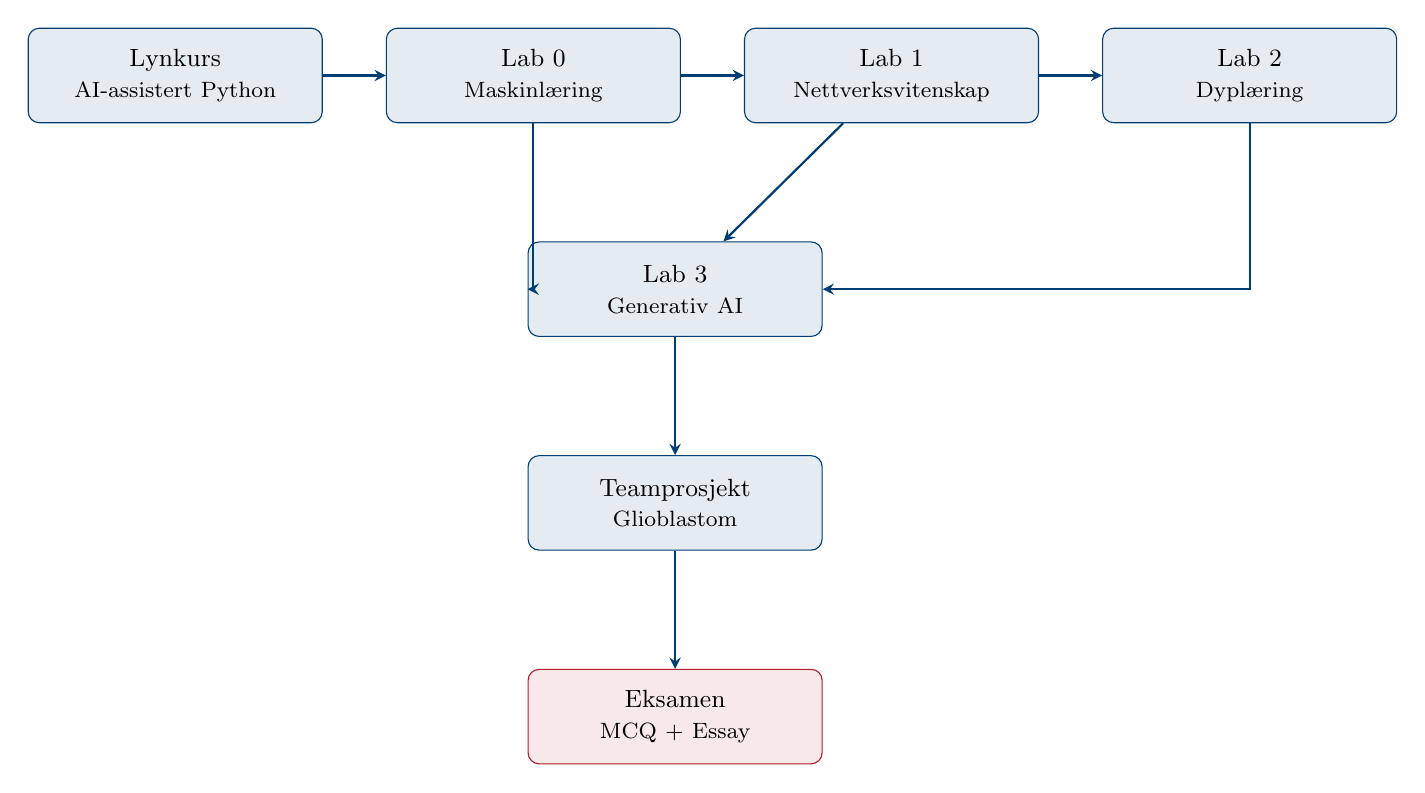
\begin{tikzpicture}[
    node distance=0.8cm,
    box/.style={rectangle, draw=uibblue, fill=uibblue!10, 
        text width=3.5cm, text centered, rounded corners, minimum height=1.2cm, font=\small},
    arrow/.style={thick,->,>=stealth,uibblue}
]
    % Row 1: Labs
    \node[box] (lynkurs) {Lynkurs\\{\footnotesize AI-assistert Python}};
    \node[box, right=of lynkurs] (lab0) {Lab 0\\{\footnotesize Maskinlæring}};
    \node[box, right=of lab0] (lab1) {Lab 1\\{\footnotesize Nettverksvitenskap}};
    \node[box, right=of lab1] (lab2) {Lab 2\\{\footnotesize Dyplæring}};
    
    % Row 2
    \node[box, below=1.5cm of lab0, xshift=1.8cm] (lab3) {Lab 3\\{\footnotesize Generativ AI}};
    
    % Row 3
    \node[box, below=1.5cm of lab3] (team) {Teamprosjekt\\{\footnotesize Glioblastom}};
    
    % Row 4
    \node[box, below=1.5cm of team, fill=uibred!10, draw=uibred] (eksamen) {Eksamen\\{\footnotesize MCQ + Essay}};
    
    % Arrows
    \draw[arrow] (lynkurs) -- (lab0);
    \draw[arrow] (lab0) -- (lab1);
    \draw[arrow] (lab1) -- (lab2);
    \draw[arrow] (lab0) |- (lab3);
    \draw[arrow] (lab1) -- (lab3);
    \draw[arrow] (lab2) |- (lab3);
    \draw[arrow] (lab3) -- (team);
    \draw[arrow] (team) -- (eksamen);
\end{tikzpicture}
\caption{Kursstruktur og progresjon i ELMED219}
\label{fig:kursstruktur}
\end{figure}

\subsection{AI i medisin -- hovedtemaer}

\begin{figure}[htbp]
\centering
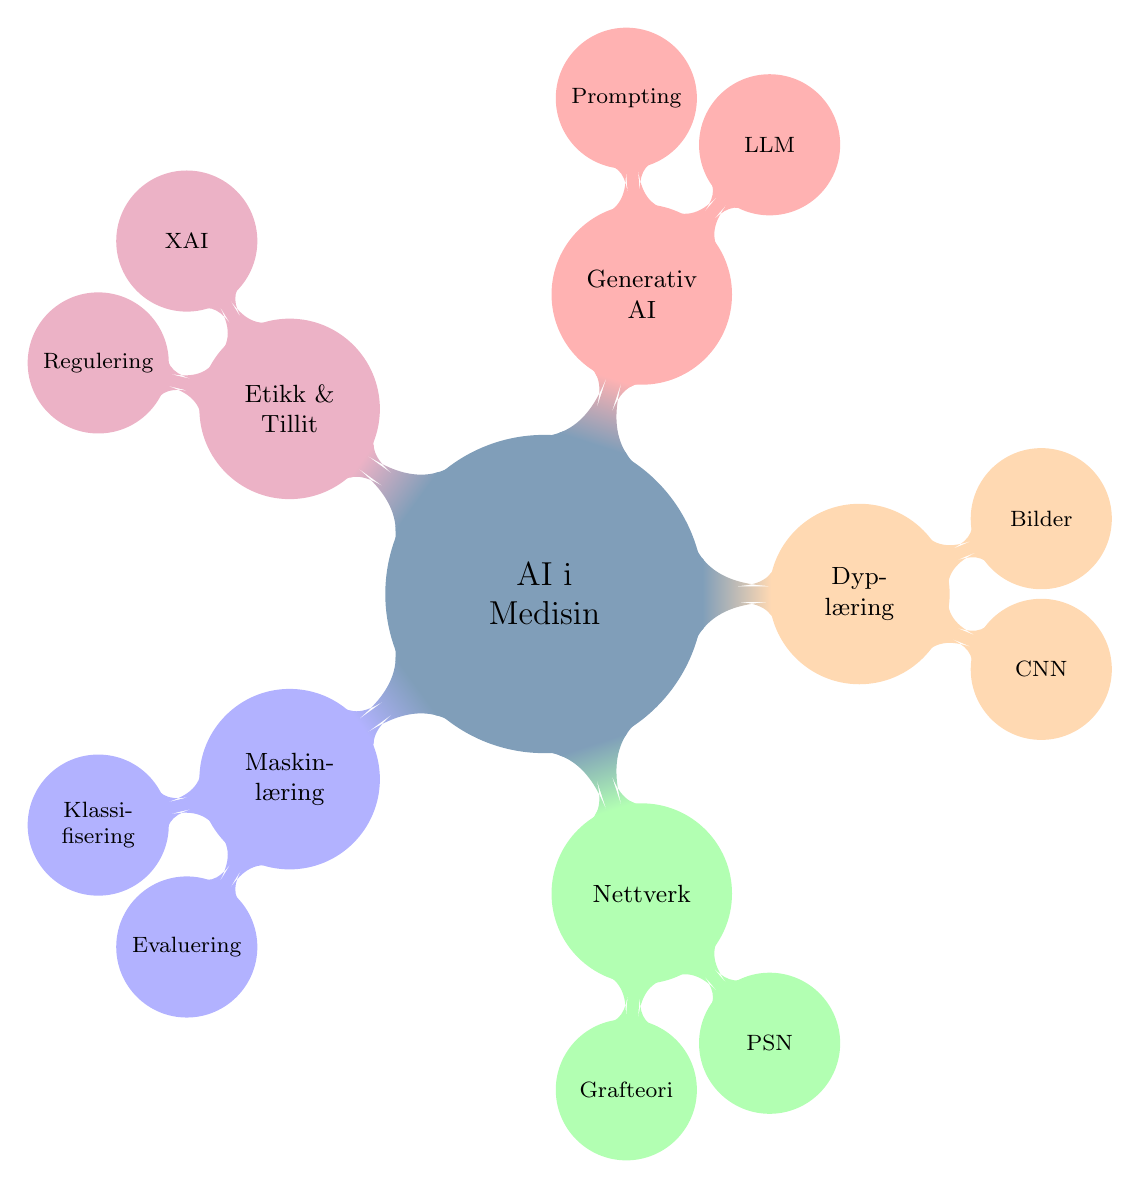
\begin{tikzpicture}[
    mindmap,
    grow cyclic,
    every node/.style={concept, execute at begin node=\hskip0pt},
    concept color=uibblue!50,
    level 1/.append style={level distance=4cm, sibling angle=72},
    level 2/.append style={level distance=2.5cm, sibling angle=45}
]
    \node[concept] {AI i\\Medisin}
        child [concept color=blue!30] { node {Maskin-\\læring}
            child { node {Klassifisering} }
            child { node {Evaluering} }
        }
        child [concept color=green!30] { node {Nettverk}
            child { node {Grafteori} }
            child { node {PSN} }
        }
        child [concept color=orange!30] { node {Dyp-\\læring}
            child { node {CNN} }
            child { node {Bilder} }
        }
        child [concept color=red!30] { node {Generativ\\AI}
            child { node {LLM} }
            child { node {Prompting} }
        }
        child [concept color=purple!30] { node {Etikk \&\\Tillit}
            child { node {XAI} }
            child { node {Regulering} }
        };
\end{tikzpicture}
\caption{Hovedtemaer i ELMED219: AI og beregningsorientert medisin}
\label{fig:temaer}
\end{figure}

\end{document}







